\documentclass[openany,oneside,a4paper,11pt]{extarticle}
% acesso a links da internet
\usepackage[pdftext]{hyperref}
\usepackage{setspace}
\usepackage[lmargin=2.5cm,tmargin=2.5cm,rmargin=2.5cm,bmargin=2.5cm]{geometry}
%\usepackage[margin=2cm,headheight=1.5cm, includeheadfoot]{geometry}
\usepackage[parfill]{parskip}
% DEFININDO OS PADRÕES DO EVENTO DA UENF
% VII Colóquio Internacional de Cognição e Linguagem

\usepackage{float}

\usepackage{graphicx}
\usepackage{subfig}
\usepackage[font=scriptsize,labelfont=bf]{caption}

\usepackage[brazil]{babel}
\usepackage[T1]{fontenc}% Selecao de codigos de fonte.
\usepackage{helvet}
\renewcommand{\familydefault}{\sfdefault}

\usepackage[table]{xcolor} % Importa o pacote para cores na tabela

\usepackage{array} % Pacote necessário para alinhamento vertical

% Cabeçalho e rodapé
%\usepackage{fancyhdr}
%\setlength\headheight{2.5cm} 
%\pagestyle{fancy}
%\lhead{}
%\chead{
%    \centering
%    
\includegraphics[width=12cm]{cabecalhoArtigoUNEF.png}
%}
%\rhead{}
%\lfoot{}
%\cfoot{\footnotesize Av. Alberto Lamego, 2000 - Parque Califórnia - Campos dos Goytacazes/ RJ\\
%Tel.: (22)  2739.7186 - Fax: (22) 2739.7281 - email: pgclcch@uenf.br }
%\rfoot{}
%\renewcommand{\headrulewidth}{0pt}

% Pacotes de citações BibLaTeX
% ----------------------------------------------------------
\usepackage[style=abnt,
	backend=biber,
	citecounter=true,
	backrefstyle=three,
	url=true,
	maxbibnames=99,
    mincitenames=1,
    maxcitenames=2,
    backref=false,
    hyperref=true,
    giveninits=true,
    uniquename=false,
    uniquelist=false]{biblatex}

% Colocar et al em itálico
\usepackage{xpatch}
\xpatchbibmacro{name:andothers}{%
  \bibstring{andothers}%
}{%
  \bibstring[\emph]{andothers}%
}{}{}

% Arquivo de entrada das referências bibliográficas
\addbibresource{referencias.bib}

% Norma NBR10.520/2023 - Sobrenomes em minúsculas
\renewcommand*{\mkbibnamefamily}[1]{#1}%
 % Norma NBR10.520/2023 - Sobrenomes em minúsculas
%\renewcommand*{\mkbibnamefamily}[1]{#1}%

%fullcite com todos autores e não como cite
\makeatletter
\newcommand{\tempmaxup}[1]{\def\blx@maxcitenames{99}#1}
\makeatother

\DeclareCiteCommand{\fullcite}[\tempmaxup]
{\usebibmacro{prenote}}
{\usedriver
	{}
	{\thefield{entrytype}}}
{\multicitedelim}
{\usebibmacro{postnote}}

\setlength\bibitemsep{12pt}

%Centralizando o Caption das imagens e tabelas
%\usepackage[justification=centering]{caption}

\usepackage{lmodern}  % Fonte compatível
\usepackage{helvet}   % Usa Arial (Helvetica)
\usepackage{setspace} % Controle de espaçamento

% Definição do subtítulo corretamente
\newcommand{\subtitle}[1]{\def\thesubtitle{#1}} 
\newcommand{\thesubtitle}{} % Inicializa o subtítulo como vazio

\makeatletter
\def\@maketitle{
    \onehalfspacing
    {\fontfamily{phv}\selectfont\fontsize{12}{12}\bfseries\centering \@title \par} % Título centralizado
    \ifx\thesubtitle\empty\else
        \vskip 1em
        {\fontfamily{phv}\selectfont\fontsize{12}{12}\bfseries\raggedright \thesubtitle \par} % Subtítulo alinhado à esquerda
    \fi
    \vskip 1em
    {\centering % Centraliza os autores
        \small
        \begin{tabular}[t]{c} % Mudança para "c" (centralizado)
            \@author
        \end{tabular}\par}
    \vskip 1em
    \eixo
    \vskip 1.5em
}
\makeatother


\title{AVANÇOS E DESAFIOS DAS INTELIGÊNCIAS ARTIFICIAIS GENERATIVAS}
\subtitle{Uma Revisão Bibliométrica sobre seus Impactos}

\author{
        Msc. Francisco Alves de Freitas Neto (IFF)\\
        francisco.freitas@gmail.com\\\\
	Dr. Carlos Henrique Medeiros (UENF)\\
        chmsouza@gmail.com\\\\
        Dr. Fabio Machado de Oliveira (UENF)\\
        fabiomac@gmail.com\\\\
        Dr. Leonard Barreto Moreira (UFF)\\
        leonardbarreto@gmail.com
        }
\usepackage{quoting}
\usepackage{abstract}
\usepackage{indentfirst}
\setlength{\parindent}{30pt} % padrão 15pt.
%\setlength{\parskip}{1cm plus 4mm minus 3mm}

\usepackage{sectsty}
\sectionfont{\fontsize{12}{15}\selectfont}
\subsectionfont{\fontsize{12}{15}\selectfont}

\usepackage{outlines}

\usepackage{longtable}

\begin{document}

\maketitle
\normalsize
\renewcommand{\baselinestretch}{1}

% ************************
% ** Resumo do trabalho **
% ************************
\renewcommand{\abstractname}{}    % clear the title
\renewcommand{\absnamepos}{empty} % originally center
%\thispagestyle{fancy}
\begin{abstract}
\noindent \normalsize \textbf{\textit{resumo - }}
Este estudo apresenta uma análise do panorama das pesquisas científicas sobre inteligências artificiais generativas (IAGs) e na forma como a comunidade acadêmica tem abordado seus impactos na sociedade. Utilizando uma revisão bibliométrica e análise de dados baseada em uma busca sistemática nas principais bases acadêmicas, o estudo mapeia o volume de publicações, os temas de maior interesse, os impactos no meio acadêmico, além das principais instituições e autores que contribuem para a área. Os resultados fornecem uma síntese estruturada das publicações sobre IAGs, servindo como um recurso para a identificação de referências qualificadas e tendências emergentes no campo.

\par \vspace{0cm}
    \noindent \textbf{Palavras-chave: }Inteligência artificial generativa, impacto, busca sistemática.

\noindent \normalsize \textbf{\textit{abstract - }}
This study presents an analysis of the landscape of scientific research on generative artificial intelligences (GAIs) and how the academic community has addressed their societal impacts. Through a bibliometric review and data analysis based on a systematic search in major academic databases, the study maps the volume of publications, key areas of interest, academic impacts, and the main institutions and authors contributing to the field. The results provide a structured synthesis of GAI-related publications, serving as a resource for identifying qualified references and emerging trends in the field.

\par \vspace{0cm}
    \noindent \textbf{Keywords: }Generative artificial intelligence, impact, systematic search.
    
\end{abstract} 

%**************
% Introdução **
%**************
\section{Introdução}
%\onehalfspacing
Nos últimos dois anos, o ambiente acadêmico tem vivenciado uma significativa popularização das tecnologias de inteligências artificiais generativas (IAGs). Como será demonstrado nas seções seguintes, essas tecnologias apresentam um potencial disruptivo no processo de pesquisa e desenvolvimento em diversas áreas do conhecimento, o que tem despertado crescente interesse da comunidade científica em investigar seus impactos.

Para ilustrar essa disrupção, \textcite{xia2024scoping} descrevem como as IAGs estão pressionando professores, alunos e instituições de ensino a revisarem seus processos avaliativos nos ambientes acadêmicos. Embora os docentes reconheçam o potencial dessas tecnologias, muitos ainda não se sentem confiantes em integrá-las como ferramenta nos métodos de avaliação.

Ainda no contexto educacional, \textcite{humble2019artificial} argumentam que essa disrupção pode ocorrer de forma mais gradual, uma vez que a adoção de IAGs tem o potencial de automatizar tarefas intelectualmente repetitivas e tediosas, permitindo que os processos genuinamente criativos permaneçam sob a responsabilidade dos humanos. Segundo os autores, o uso de IAGs estreitas\footnote{Os autores reforçam os conceitos de IAGs estreitas, que são aquelas capazes de aplicar métodos dedutivos e indutivos sobre a base de conhecimento utilizada no processo de aprendizagem, em contraste com as IAGs gerais, que se distinguem por sua capacidade de gerar hipóteses de forma criativa, utilizando métodos abdutivos.}, sejam fortes ou fracas, para atividades que demandam criatividade pode levar à frustração, seguida por um ajuste das expectativas e uma compreensão mais realista de suas reais capacidades.

Segundo os autores \textcite{ifenthaler2024artificial}, o uso responsável das IAGs deve enfatizar o conceito de \textit{man in the loop}, que propõe que a remoção da presença humana central nos processos de ensino e aprendizagem é um equívoco. Para os autores, a adoção ética dessas tecnologias, preservando as privacidades intelectuais, com a utilização de algoritmos confiáveis e garantindo acesso igualitário, é essencial para assegurar uma prática educacional confiável, mesmo que isso requeira uma revisão dos métodos de ensino e aprendizagem.

O que todos os autores mencionados têm em comum é a compreensão de que os profissionais de educação precisam estar cientes das potencialidades oferecidas por essas tecnologias. Parte das dificuldades enfrentadas no processo de ensino e aprendizagem decorre da falta de clareza sobre o funcionamento das IAGs e de como esses processos podem ser efetivamente aplicados nas atividades acadêmicas sem comprometer os processos de ensino, aprendizagem e avaliação. Essas dificuldades também se devem ao caráter inovador de uma tecnologia que, até recentemente, era exclusiva da humanidade: a produção de textos com significado. Esse processo demanda um esforço intelectual e cultural desenvolvido ao longo da história. Diferentemente da fala, a leitura e, consequentemente, a escrita exigem aprendizado e domínio de mecanismos culturais, habilidades intelectuais, empáticas e motoras que permitem a construção e interpretação de textos \cite{Wolf2019}. De acordo com Maryanne Wolf, esse aprendizado é um processo artificial, profundamente ligado à capacidade de manipular as tecnologias de cada época. Assim, a adaptação a novas ferramentas não deve ser vista como algo surpreendente no contexto da produção textual.

Neste sentido, este artigo apresenta uma seção dedicada aos fundamentos teóricos das IAGs. Esses modelos representam um marco significativo no desenvolvimento tecnológico, impulsionando a popularização dessas tecnologias como ferramentas de apoio em diversas atividades que, até recentemente, eram exclusivas da cognição humana. Considerando que a pesquisa se concentra nos impactos das IAGs nas atividades intelectuais humanas, o artigo abordará de maneira mais aprofundada os modelos geradores de linguagem textual, conhecidos como \textit{Large Language Models} (LLM), pois são, de longe, os mais populares e, portanto, os que causam o maior impacto atualmente.

%Definição dos objetivos
Como será apresentado neste artigo, o crescente volume de publicações na área de IAGs torna desafiadora a identificação de informações que caracterizem com precisão o impacto dessas tecnologias em diferentes atividades humanas. Nesse contexto, a organização das publicações por meio de uma busca sistemática, fundamentada em critérios bibliométricos e de ciência de dados, permite avaliar a qualidade dos estudos e extrair novas informações a partir dos dados analisados. Essa abordagem contribui para a construção de fundamentações rigorosas e amplamente aceitas pela comunidade científica, garantindo maior confiabilidade aos estudos futuros \cite{ferreira2010bibliometria}.

O principal objetivo deste artigo é examinar o panorama das pesquisas científicas sobre inteligências artificiais generativas (IAGs) e seus impactos em distintas áreas do conhecimento, bem como consolidar um referencial composto por publicações de qualidade que contribuam para a investigação dos efeitos dessas tecnologias na sociedade contemporânea. Para esse fim, a seção de fundamentação teórica apresentará uma síntese dos conceitos bibliométricos que embasam a metodologia adotada, delineando os critérios e abordagens empregados na análise do corpus bibliográfico.

Com a aplicação das técnicas de bibliometria previamente descritas, busca-se estabelecer uma base de referências robusta, além de um catálogo abrangente das principais instituições e autores que contribuem para a pesquisa sobre inteligências artificiais generativas (IAGs). Adicionalmente, a análise das relações de citação entre publicações e a frequência dos termos empregados permitirá identificar os conceitos mais recorrentes, evidenciando os principais focos de interesse na literatura acadêmica. Por fim, este estudo pretende responder às seguintes questões norteadoras:

\begin{itemize}
    \item Quais são os principais centros difusores da pesquisa sobre os impactos das IAGs?
    \item Quais são os autores mais produtivos nessa abordagem?
    \item Em quais áreas do conhecimento são publicados mais artigos relevantes?
\end{itemize}

%Início da metodologia
Para atingir o objetivo de construir uma base bibliográfica sólida e confiável, este estudo inicia-se com uma pesquisa exploratória, baseada na consulta a referenciais teóricos e documentais. Além disso, adota-se uma abordagem quantitativa e qualitativa sobre o tratamento das bases de dados de artigos, conforme descrito por \textcite{carlosHenrique2010Metodologia, gil2002elaborar}, utilizando metodologia bibliométrica para a análise de dados provenientes das bases de publicações científicas Web of Science, Scopus e IEEE. 

A Figura \ref{fig:metodologias} apresenta uma visão geral dos procedimentos metodológicos bibliométricos adotados. O diagrama destaca a aplicação das leis de Bradford, Lotka e Zipf, utilizadas, respectivamente, para selecionar os periódicos mais relevantes, identificar os autores mais produtivos e mapear os temas predominantes. Cada etapa de filtragem foi recuperada e integrada ao processo subsequente, permitindo a construção progressiva de um conjunto refinado de artigos relevantes ao final da análise.

\begin{figure}[H]
    \centering
    \caption{Diagrama com as metodologias adotadas na pesquisa}
    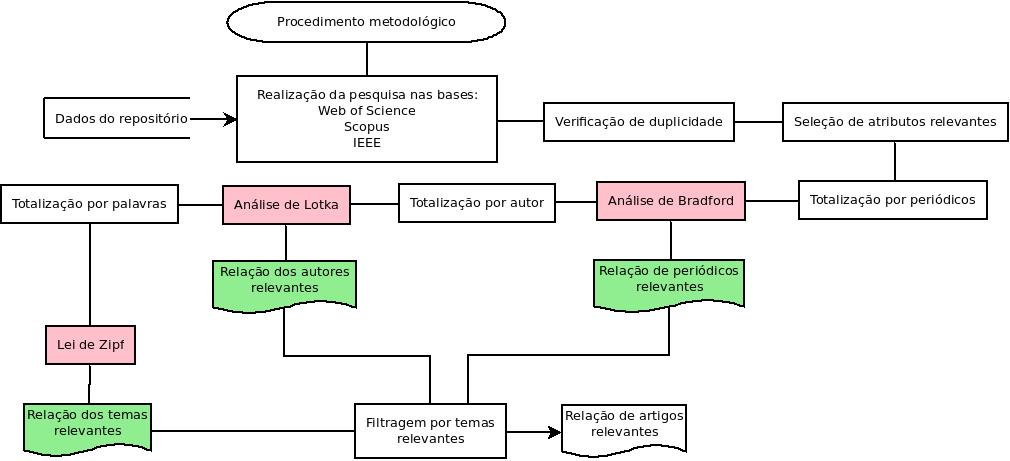
\includegraphics[width=16cm]{Procedimento_metodologico_visao geral.jpeg}
    \label{fig:metodologias}
    {\\\footnotesize Fonte: Autoria Própria}
\end{figure}

A seção "Desenvolvimento do Tema"  detalhará os procedimentos metodológicos adotados, os resultados obtidos e as contribuições de cada etapa do estudo. Serão discutidos os critérios que fundamentaram a escolha do tema final, orientando a seleção dos artigos analisados. Além disso, essa seção apresentará um resumo das publicações selecionadas, destacando os principais aspectos abordados por cada uma delas.

%Início da fundamentação teórica
\section{Fundamentação Teórica}

Para fundamentar teoricamente esta pesquisa, considerando seu caráter interdisciplinar, esta seção foi estruturada em duas partes, cada uma abordando distintas áreas do conhecimento. A primeira subseção apresenta os conceitos fundamentais sobre inteligência artificial, com ênfase nas redes neurais artificiais. A segunda subseção trata dos princípios da bibliometria, incluindo a definição e aplicação das Leis de Bradford, Lotka e Zipf, previamente mencionadas na Introdução. Por fim, busca-se estabelecer a relação entre esses temas, demonstrando como a abordagem bibliométrica pode contribuir para a análise dos impactos das IAGs e da forma como a academia tem explorado essa temática.

\subsection{Inteligência Artificial Generativa}

O termo Inteligência Artificial (IA), embora de definição ampla, tornou-se um dos temas centrais nas discussões contemporâneas. Nos últimos cinco anos, observou-se um avanço significativo nessas tecnologias, impulsionado pelo crescente uso de IAs preditivas baseadas em Redes Neurais Artificiais (RNAs) e, mais recentemente, pelo desenvolvimento das Redes Neurais Generativas (RNAGs).

Definir IA pode ser uma tarefa complexa. \textcite{lugerIA_2004} explica que essa dificuldade é justificável, pois a própria definição de inteligência em organismos vivos é um desafio conceitual. O autor destaca que, ao observar um agente inteligente, seja ele natural ou artificial, percebe-se que seu comportamento reflete uma autonomia responsiva a determinadas condições, sugerindo uma intencionalidade mais complexa do que a simples aleatoriedade probabilística.

Outros autores, como \textcite{haykin1999neural}, descrevem a IA como um conjunto de artefatos algorítmicos projetados para simular o pensamento humano em tarefas específicas. Já \textcite{silva2016redes}, ao aplicar a IA na resolução de problemas práticos na engenharia, a interpreta como uma ferramenta para lidar com questões complexas e de difícil modelagem matemática, incluindo análise de imagens, reconhecimento de padrões de escrita e fala, biometria e previsão de mercado financeiro, entre outras aplicações.

Independentemente da concepção adotada para definir uma IA, ou mais especificamente uma IAG, pode-se afirmar com segurança que essas tecnologias estão sempre associadas a uma rede neural artificial treinada em extensas bases de dados, conhecidas como \textit{big data}. Como resultado desse treinamento, a saída gerada consiste em sequências de dados que podem ser interpretadas como novos textos produzidos.

\begin{quoting}[rightmargin=0cm,leftmargin=4cm]
{\footnotesize 
\begin{singlespace}
\noindent
A IA generativa (IAG) é uma área da inteligência artificial que se dedica em criar soluções, conteúdos e dados novos, a partir de informações armazenadas em grandes bases de dados. Vale notar que a criação executada pela IA generativa tem como base os produtos que já foram concebidos pela mente humana \cite[Pág. 121]{hessel2023criatividade}.
\end{singlespace}
}
\end{quoting}

Segundo \textcite{lugerIA_2004}, uma rede neural artificial é uma técnica de inteligência artificial que busca reproduzir, de forma simplificada, o funcionamento de um sistema biológico de neurônios naturais. Embora essa abordagem não seja recente, suas origens estão intimamente ligadas à história da computação. Os primeiros modelos conexionistas foram propostos em 1943 pelos matemáticos Warren McCulloch e Walter Pitts, baseando-se na ativação de neurônios artificiais por meio do acúmulo de estímulos em suas entradas, resultando em uma saída determinada por uma função matemática de ativação.

Esse comportamento apresenta semelhanças, em menor escala, com o funcionamento dos neurônios biológicos, que, ao receberem estímulos elétricos nos dendritos, podem gerar impulsos ao longo do axônio. A Figura \ref{fig:2} ilustra essas correspondências estruturais e funcionais. De maneira geral, tanto as redes neurais artificiais quanto as biológicas são formadas por múltiplas camadas de neurônios interconectados, cujas conexões, denominadas sinapses, desempenham um papel fundamental no processamento e na transmissão das informações.

\begin{figure}[h]
    \centering
    \caption{Comparação entre os modelos neurais biológicos e artificiais}    
    \subfloat[Representação de um neurônio natural]{%
        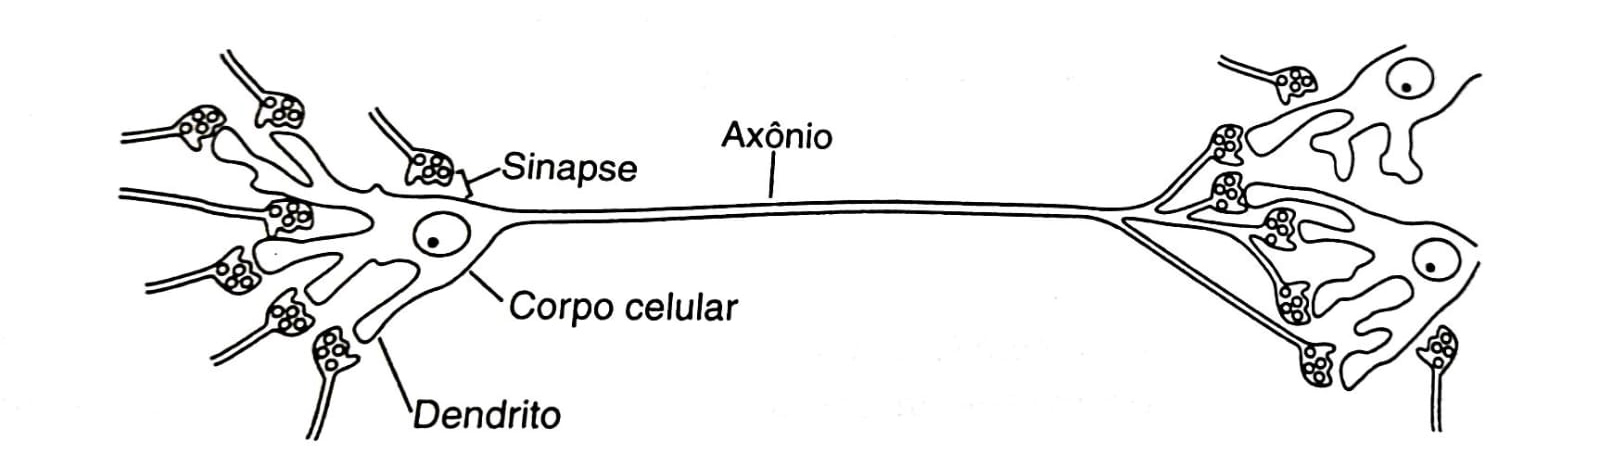
\includegraphics[width=0.6\textwidth]{IMG-20241018-WA0020.jpg}
        \label{fig:2.1}
        }
    \quad
    \subfloat[Representação de um neurônio artificial]{%
        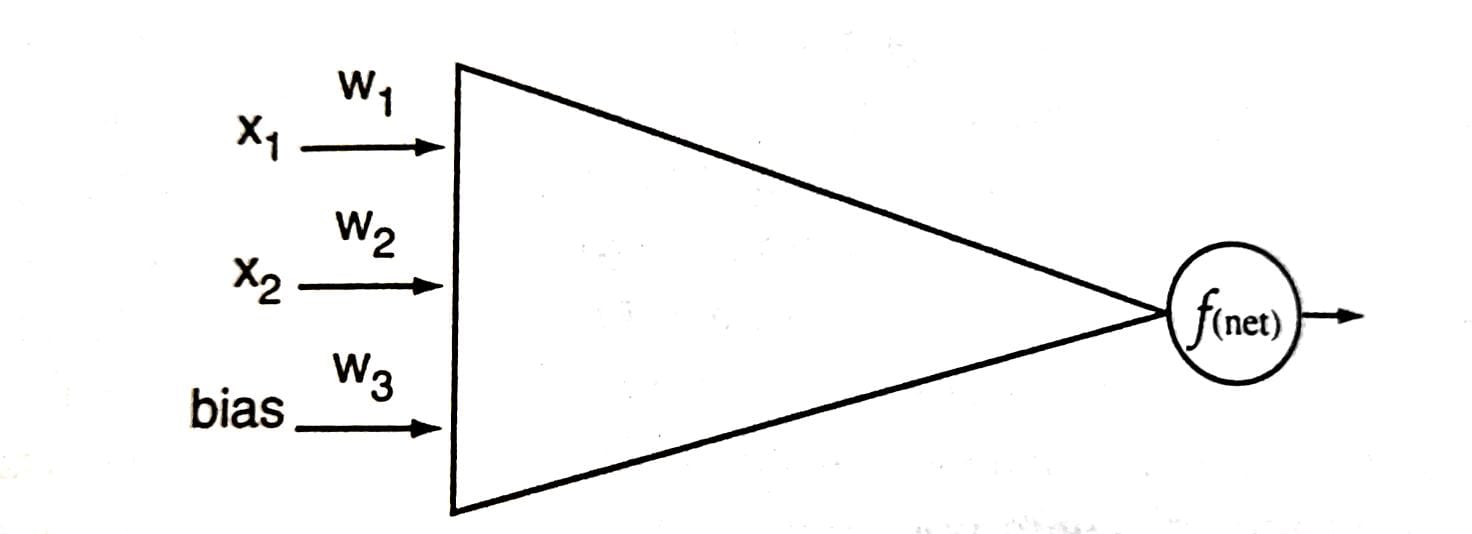
\includegraphics[width=0.6\textwidth]{IMG-20241018-WA0021.jpg}
        \label{fig:2.2}
        }
    \label{fig:2}
    {\\\footnotesize Autor: \cite{lugerIA_2004}[pags. 46, 399]}
\end{figure}

Os modelos conexionistas possuem a capacidade de ajustar seus pesos sinápticos, representados por valores como \( w_1, w_2, w_3 \), de modo a convergir para um padrão de saída específico. Esse ajuste ocorre por meio da minimização do erro em relação aos resultados esperados ou da otimização dos pesos para maximizar o desempenho do modelo. Esse processo adaptativo, fundamental para a melhoria contínua da rede, é conhecido como aprendizado de máquina (\textit{Machine Learning}), conforme discutido por \textcite{haykin1999neural}.

Mais especificamente, as Redes Neurais Artificiais Generativas (RNAGs) de texto empregam um processo de aprendizado de máquina não supervisionado, no qual a atualização dos pesos das conexões ocorre com base na comparação entre as respostas geradas e os textos selecionados dentro de um determinado contexto. Assim, caso a máquina não produza uma resposta adequada a um estímulo, o processo de aprendizado é repetido, ajustando os parâmetros até que a escolha das palavras na resposta reflita padrões estatísticos previsíveis. Esse mecanismo caracteriza um aprendizado autônomo, no qual a máquina aprimora suas respostas por meio da interação contínua com os dados.

Em relação a produtos como o ChatGPT, que empregam modelos de processamento de linguagem natural (\textit{Natural Language Processing} - NLP), a arquitetura \textit{Transformer} é a mais comumente adotada. De acordo com \textcite{vaswani2017attention}, esses modelos oferecem maior capacidade de processamento por eliminarem as recorrências complexas dos modelos anteriores, permitindo maior paralelização e, portanto, melhorando a eficiência de desempenho. O autor explica que essa arquitetura opera analisando uma sequência de palavras como entrada e produzindo uma sequência como saída. Essa análise da sequência é dividida em duas componentes principais: \textit{encoder} e \textit{decoder}, ambas ilustradas na Figura \ref{fig:transformer}.

\begin{figure}[h]
    \centering
    \caption{Descrição da Arquitetura Transformer}
    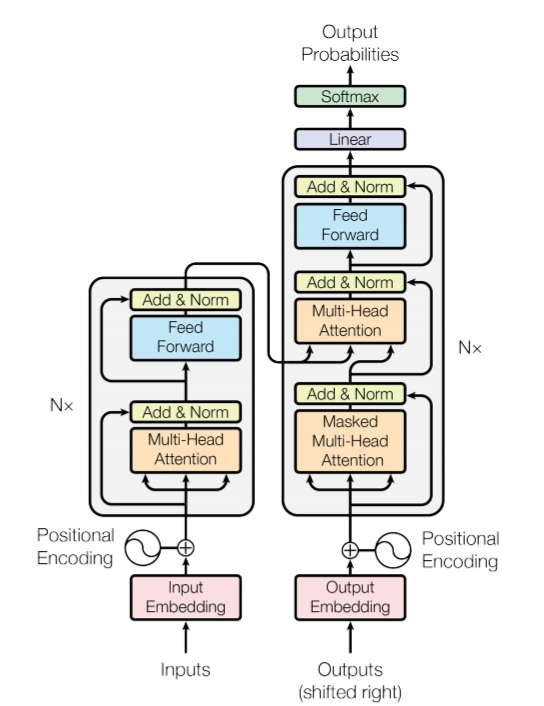
\includegraphics[width=11cm]{modeloTransformer.jpg}
    \label{fig:transformer}
    {\\\footnotesize Autor: \cite[pág. 3]{vaswani2017attention}}
\end{figure}

O módulo \textit{encoder}, posicionado à esquerda, tem a função de generalizar a entrada das palavras do texto fornecido pelo usuário, buscando extrair seu significado. Por outro lado, o \textit{decoder}, situado à direita, é encarregado de escolher a sequência de palavras que constituirão a resposta. Este procedimento envolve um cálculo de otimização para determinar a palavra mais provável a ser produzida. Desta maneira, os sistemas de PLN atuam como máquinas que geram textos com base em cálculos estatísticos, usando suas bases de treinamento — ou \textit{big data} inicial. Assim, não se deve esperar que os textos gerados ultrapassem os contextos que não foram assimilados durante o período de treinamento.
\subsection{Conceitos de Bibliometria}
Segundo \textcite{gracio2020topicos}, a bibliometria têm se consolidado como campo de estudo fundamental para a compreensão da natureza e da avaliação da comunicação científica. Ainda segundo este autor, a bibliometria, por meio de seus métodos quantitativos, pode subsidiar processos decisórios, alinhando-se à qualificação do pesquisador, para formar um material de consulta bibliográfica de qualidade. Portanto, a aplicação da bibliometria no desenvolvimento de uma base de publicações sobre o tema de IAGS, fornece um método objetivo para identificar deficiências informacionais, como a obsolescência de ideias, autores e termos indexados, além do uso de neologismos, muito comum em temas tecnológicos, e a identificação de áreas em ascensão ou declínio.

A bibliometria é fundamentada em três leis principais: a Lei de Bradford, que trata da produtividade dos periódicos; a Lei de Lotka, que aborda a produtividade dos autores; e a Lei de Zipf, que analisa a frequência de ocorrência de palavras \cite{ferreira2010bibliometria}. Dado que este estudo visa construir uma base de referências para consulta de publicações, torna-se essencial identificar fontes confiáveis de artigos científicos, como congressos e universidades. Nesse contexto, a Lei de Bradford desempenha um papel central na condução da pesquisa bibliométrica.

A Lei de Bradford, também denominada Lei de Dispersão, permite quantificar a produtividade dos periódicos e identificar tanto o núcleo quanto as áreas de dispersão de um determinado tema dentro de um conjunto de publicações. Segundo essa lei, os primeiros estudos sobre um novo tema tendem a ser submetidos a um número reduzido de revistas especializadas que, ao aceitá-los, atraem um volume crescente de publicações relacionadas à temática ao longo do tempo. Simultaneamente, outras revistas começam a publicar seus primeiros manuscritos sobre o assunto, criando outras possíveis áreas de dispersão. Caso a área continue a se desenvolver, consolida-se um núcleo de periódicos mais produtivos, responsáveis por concentrar a maior parte dos estudos sobre o tema \cite{lousada2012produccao}.

Além de identificar fontes confiáveis para as referências da pesquisa, é igualmente importante compreender a relevância dos autores nas produções acadêmicas, considerando aspectos como a quantidade de artigos publicados sobre o tema, sua produtividade, citações, entre outros. Nesse contexto, a Lei de Lotka se torna crucial para esta investigação. A seguir, apresenta-se a descrição dessa lei:

A Lei de Lotka, também conhecida como Lei do Quadrado Inverso, descreve a distribuição da produtividade dos pesquisadores, utilizando um modelo de distribuição tamanho-frequência dos pesquisadores em um conjunto de artigos. Em termos práticos, a produtividade de um autor, medida pelo número de artigos publicados, reflete a sua contribuição para o avanço do conhecimento científico. Estudada por Lotka (1926), essa lei afirma que o número de pesquisadores que fazem $n$ contribuições em um determinado campo do conhecimento científico é aproximadamente $1/n^2
$ do número de pesquisadores que fazem apenas uma contribuição. Além disso, a proporção dos pesquisadores que contribuem com apenas um artigo gira em torno de 60\% \cite{melo2017bibliometria}. A Lei de Lotka pode ser calculada utilizando a fórmula apresentada pela equação \ref{eq:lotka}.

\begin{equation}
a_n = a_1 \cdot \frac{1}{n^c}
\label{eq:lotka}
\end{equation}

onde:
\begin{itemize}
    \item \( a_n \) é o número de autores com \( n \) artigos,
    \item \( a_1 \) é o número de autores que publicaram apenas um artigo,
    \item \( c \) é o coeficiente de Lotka.
\end{itemize}

Como descrito na equação \ref{eq:lotka}, o número de autores diminui conforme o número de artigos aumenta.

Esta pesquisa bibliométrica visa orientar os pesquisadores sobre as palavras mais frequentes nas publicações, razão pela qual a Lei de Zipf será abordada neste estudo. A Lei de Zipf, proposta em 1949 e também conhecida como a "lei do mínimo esforço", analisa a frequência de ocorrência das palavras em um texto. Para isso, gera-se uma lista com as palavras presentes no texto, organizadas em ordem decrescente de acordo com sua frequência de ocorrência. A posição de cada palavra nesta lista é denominada ordem de série ou \textit{rank}. Zipf desdobrou sua proposta original em duas vertentes: a primeira, aplicada exclusivamente às palavras de alta frequência; e a segunda, modificada por Andrew Boot, que propõe que várias palavras com baixa frequência de ocorrência compartilham a mesma posição em determinado texto \cite{gracio2020topicos}.

%*************** Desenvolvimento do tema **********************
\section{Desenvolvimento do tema}

Na seção de Introdução do presente estudo, é exibido um diagrama na Figura \ref{fig:metodologias} que ilustra a sequência metodológica a ser adotada ao longo da pesquisa. Para uma compreensão mais detalhada das ações descritas nesta seção, as etapas de pesquisa e seus respectivos resultados, quantitativos e qualitativos, serão apresentados minuciosamente, seguindo a ordem sequencial demonstrada na figura referida.

Conforme descrito por \textcite{zupic2015bibliometric}, para o levantamento de dados desta investigação, foi aplicado um filtro na seleção de publicações nas seguintes bases de indexação: Web of Science; Scopus; e IEEE. Os termos utilizados foram "Generative Artificial Intelligence" ou "Artificial Intelligence", em combinação com "Impact". A Tabela \ref{tab:publicacoes} demonstra as buscas realizadas em cada base e o número de resultados obtidos.

\begin{table}[H]
    \centering
    {%\footnotesize
    \begin{tabular}{c>{\raggedright\arraybackslash}m{10cm}c}
        \hline
        \textbf{Base} & \textbf{Comando} & \textbf{Publicações} \\
        \hline
        Web of Science & ((ALL=(impact)) AND(ALL=("Artificial Intelligence") OR ALL=("Generative Artificial Intelligence")) & 46.416 \\\hline
        Scopus & ALL ( "Impact" ) AND ( ALL ( "Artificial Intelligence" ) OR ALL ( "Generative Artificial Intelligence" ) ) & 813,496 \\\hline
        IEEE & (("All Metadata":"impact") AND ("All Metadata":"Artificial Intelligence" OR "All Metadata":"Generative Artificial Intelligence")) & 14.689 \\
        \hline
    \end{tabular}
    }
    \caption{Consulta de publicações sobre Inteligências Artificiais Generativas e seus impactos}
    \label{tab:publicacoes}
\end{table}

Embora o Scopus apresente uma quantidade maior de publicações, as três bases de dados escolhidas oferecem um número suficientemente representativo de registros para análise. Considerando também as limitações de navegação de cada sistema, a exportação de dados foi conduzida obedecendo ao limite padrão de 1.000 registros por base, ordenados por relevância, garantindo assim uma amostra relevante para o estudo.

A partir dos dados brutos disponibilizados, realizou-se uma análise quantitativa das publicações anuais, conforme demonstrado na Figura \ref{fig:2}. Na amostra examinada, observou-se claramente que, devido à recente influência das IAGs na sociedade, o volume de publicações nas três bases de dados estudadas tornou-se significativo apenas a partir de 2018. Este ano foi, portanto, adotado como limite inferior para a análise. Com essa delimitação temporal, a amostra original, que contava com 3000 artigos, foi reduzida para 2945 publicações. Adicionalmente, identificou-se que a base de dados Scopus registrou o maior número de publicações relevantes, salientando-se a partir do ano de 2023.

\begin{figure}[H]
    \centering
    \caption{Comparativo do volume de publicações ao longo do tempo, nas base: Web of Science, Scopus e IEEE.}
    \subfloat[Comparativo total das publicações]{%
        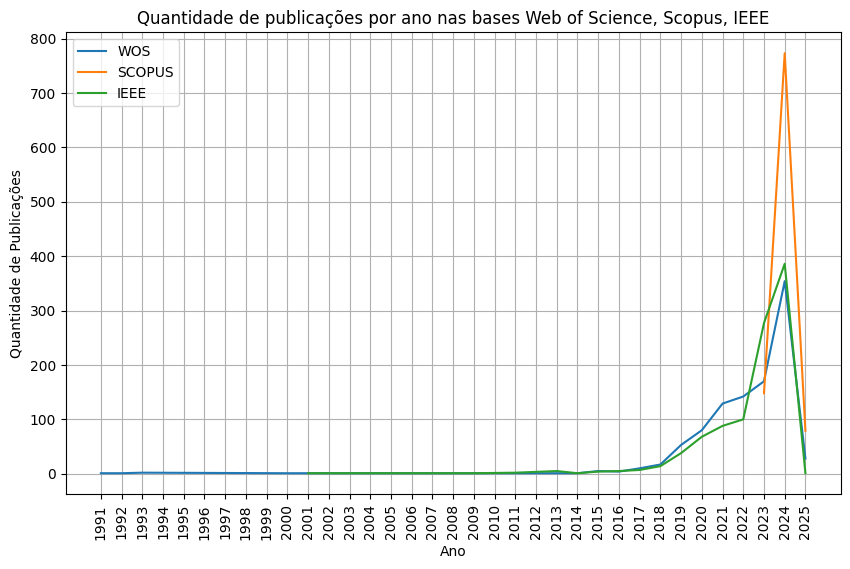
\includegraphics[width=13cm]{comparativo_volume_de_publicacoes_geral.png}
        \label{comp.publicacoes1}
    }
    \quad
    \subfloat[Comparativo das publicações a partir de 2018]{%
        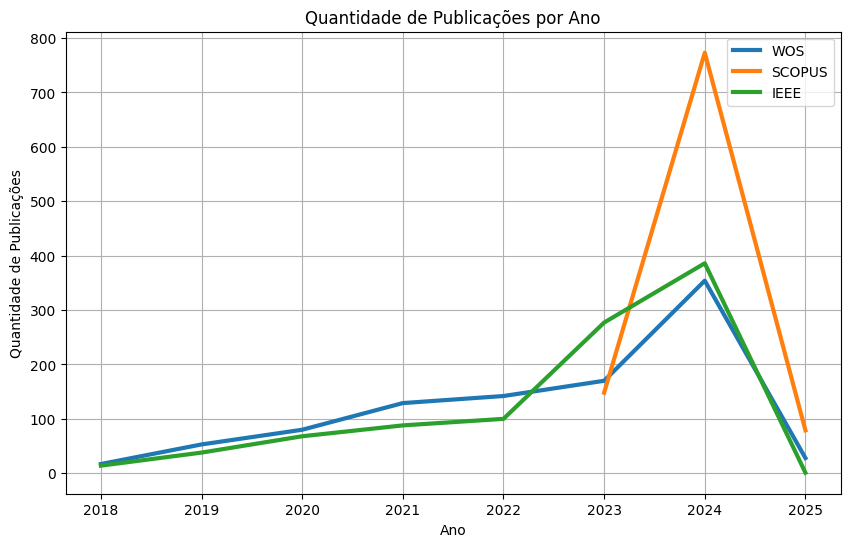
\includegraphics[width=13cm]{Comparativo_volume_de_publicações_impacto.png}
        \label{comp.publicacoes2}
    }
    {\\\footnotesize Fonte: Autoria Própria}
    \label{fig:2}
\end{figure}

Após remover duplicidades de registros e corrigir erros nos cadastros, a análise foi restringida a 2838 artigos distribuídos por 1844 periódicos. Esses números sugerem uma considerável quantidade de publicações ainda em debate, possivelmente indicando um campo acadêmico em avanço contínuo sem a predominância de revistas amplamente reconhecidas. Tópicos mais estabelecidos frequentemente possuem publicações especializadas, resultando em um menor número de periódicos abordando esses temas \cite{lousada2012produccao}.

%***** Subsecção da produtividade dos periódicos *****
\subsection{Análise da produtividade dos periódicos}

Para aprofundar a compreensão acerca da origem das publicações e reconhecer os principais responsáveis pela disseminação de artigos relativos ao tópico em questão, procedeu-se à concatenação dos dados provenientes das três bases de dados distintas. Posteriormente, foi implementado um método de agrupamento com o propósito de examinar detalhadamente as fontes dessas publicações. Os achados resultantes dessa análise estão visualmente representados no gráfico apresentado na Figura \ref{fig:3}.

\begin{figure}[H]
    \centering
    \caption{Análise quantitativa parcial de publicações por sua origem}
    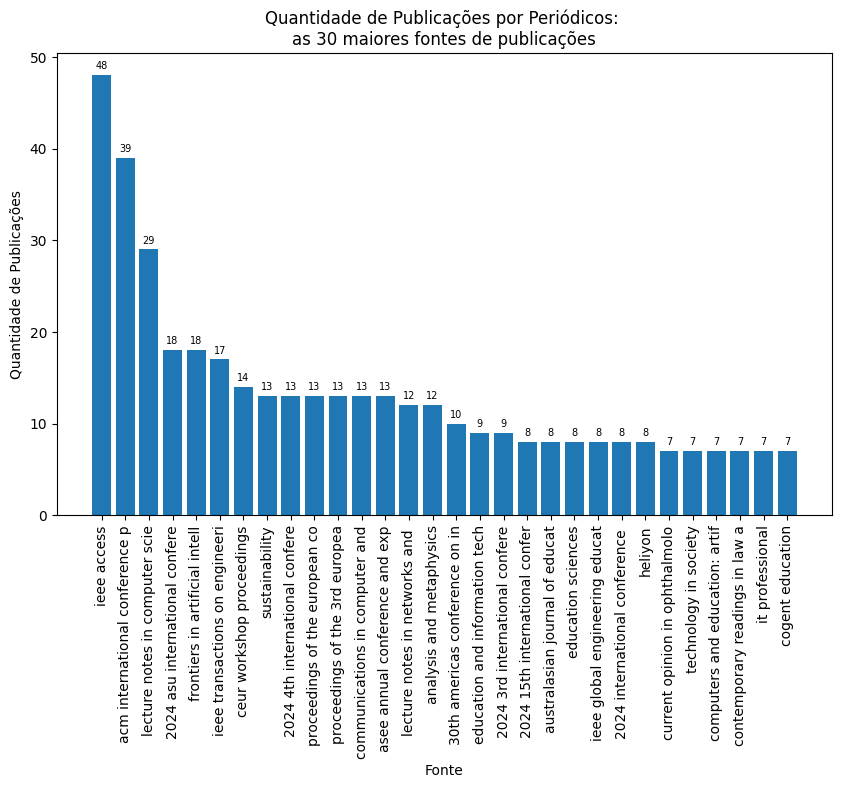
\includegraphics[width=13cm]{qtd_publicacoes_fonte.png}
    {\\\footnotesize Fonte: Autoria Própria}
    \label{fig:3}
\end{figure}

Como era previsto, dada a vasta quantidade de periódicos incluídos na amostra e considerados de importância, a análise apresentada na Figura \ref{fig:3} indica uma dispersão significativa das publicações através de múltiplos periódicos. Existem alguns periódicos que, exibindo um alto índice de disseminação, acumulam um número considerável de publicações, contudo, este número permanece relativamente baixo quando comparado ao total de artigos relevantes publicados no conjunto da amostra.

A tabela \ref{tab:resumo_qtd_publicacoes} fornece uma totalização abrangente das publicações consideradas, incluindo a quantidade de periódicos ligados a cada total. É nitidamente evidente que, conforme o número de publicações atribuídas a cada periódico diminui, há um aumento no número de fontes responsáveis por sua disseminação. Assim, pode-se inferir que as fontes que apresentam um menor volume de publicações tendem a ser menos relevantes no contexto do tema investigado \cite{lousada2012produccao}.

\begin{table}[H]
    \centering
    %{%\fontsize{6pt}{7pt}\selectfont
    \begin{tabular}{cccc}
        \hline
        Qtd. Publicações & Qtd. Fontes & Total Fontes & Total Publicações \\
        \hline
        \rowcolor{red!30} 48  & 1    & 1    & 48   \\
        \rowcolor{red!30} 39  & 1    & 2    & 87   \\
        \rowcolor{red!30} 29  & 1    & 3    & 116  \\
        \rowcolor{red!30} 18  & 2    & 5    & 152  \\
        \rowcolor{red!30} 17  & 1    & 6    & 169  \\
        \rowcolor{red!30} 14  & 1    & 7    & 183  \\
        \rowcolor{red!30} 13  & 6    & 13   & 261  \\
        \rowcolor{red!30} 12  & 2    & 15   & 285  \\
        \rowcolor{red!30} 10  & 1    & 16   & 295  \\
        \rowcolor{red!30} 9   & 2    & 18   & 313  \\
        \rowcolor{red!30} 8   & 6    & 24   & 361  \\
        \rowcolor{red!30} 7   & 9    & 33   & 424  \\
        \rowcolor{red!30} 6   & 12   & 45   & 496  \\
        \rowcolor{red!30} 5   & 12   & 57   & 556  \\
        \rowcolor{red!30} 4   & 27   & 84   & 664  \\
        \rowcolor{red!30} 3   & 81   & 165  & 907  \\
        2   & 252  & 417  & 1411 \\
        1   & 1427 & 1844 & 2838 \\
        \hline
        %}
    \end{tabular}
    \caption{Tabela de publicações e periódicos com destaque para os periódicos relevantes.}
    \label{tab:resumo_qtd_publicacoes}
\end{table}

Na subsequente fase do estudo, realizou-se a análise de dispersão das publicações com o objetivo primordial de identificar os grupos responsáveis pela difusão do conhecimento, em cumprimento ao enunciado da Lei de Bradford \cite{gracio2020analises} e \cite{lousada2012produccao}. Para tal análise, as fontes dos artigos científicos foram classificadas em três categorias distintas, com a ordenação baseada no volume de publicações. A distribuição seguiu um método que consiste em dividir o total de publicações em três partes iguais, resultando em um valor de referência de $2838/3 = 946$. O núcleo de Bradford, caracterizando as fontes mais influentes e significativas, é representado pelo conjunto de publicações até a linha evidenciada na Tabela \ref{tab:resumo_qtd_publicacoes}. Assim, pode-se constatar que, para cada periódico incluído na categoria mais influente, existem doze outros com menor relevância, demonstrando claramente a concentração da produção científica em 165 periódicos de elevado impacto.

Com base nas teorias dos núcleos de difusores propostas por Bradford, tornou-se viável identificar um conjunto de periódicos que possuem maior relevância para a pesquisa, permitindo a redução da base inicial de 2838 publicações para um total de 907 artigos considerados apropriados para análise detalhada. É importante destacar que este procedimento de filtragem revela ainda mais claramente que o tema investigado continua sendo altamente inovador. Como ilustrado na Figura \ref{fig:perio_public}, é perceptível que uma grande parte dos periódicos selecionados após a aplicação do critério de corte apresentam apenas três artigos publicados.

\begin{figure}[H]
    \centering
    \caption{Análise quantitativa de periódicos por quantidade de publicações}
    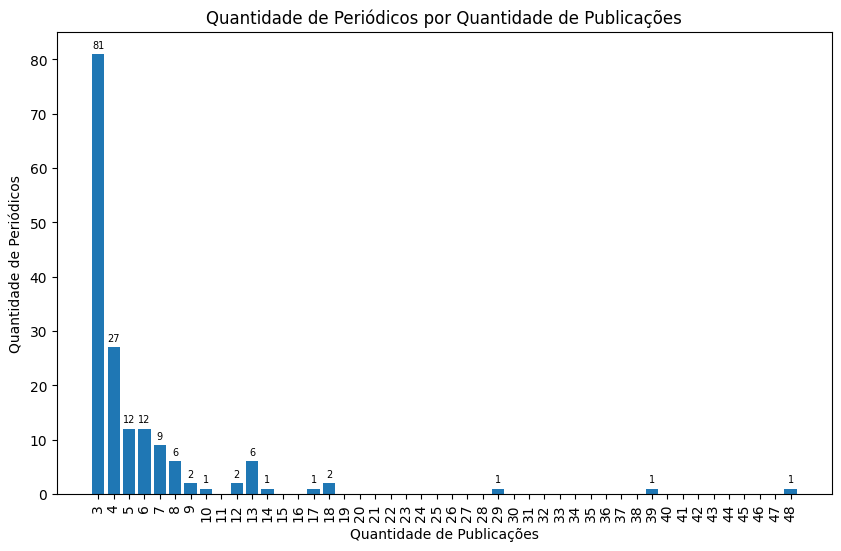
\includegraphics[width=13cm]{elite_bradford.png}
    {\\\footnotesize Fonte: Autoria Própria}
    \label{fig:perio_public}
\end{figure}

%**** Subseção da produtividade dos autores ****
\subsection{Análise da produtividade dos autores}
Utilizando a base de dados composta por 907 artigos, conforme obtido na subseção anterior, foi adotada uma metodologia similar à previamente descrita para investigar o volume de produção de cada autor em cada uma das bases de dados analisadas. Os resultados parciais dessa investigação estão ilustrados na Figura \ref{fig:4}.

\begin{figure}[H]
    \centering
    \caption{Totalização de publicações por autores}
    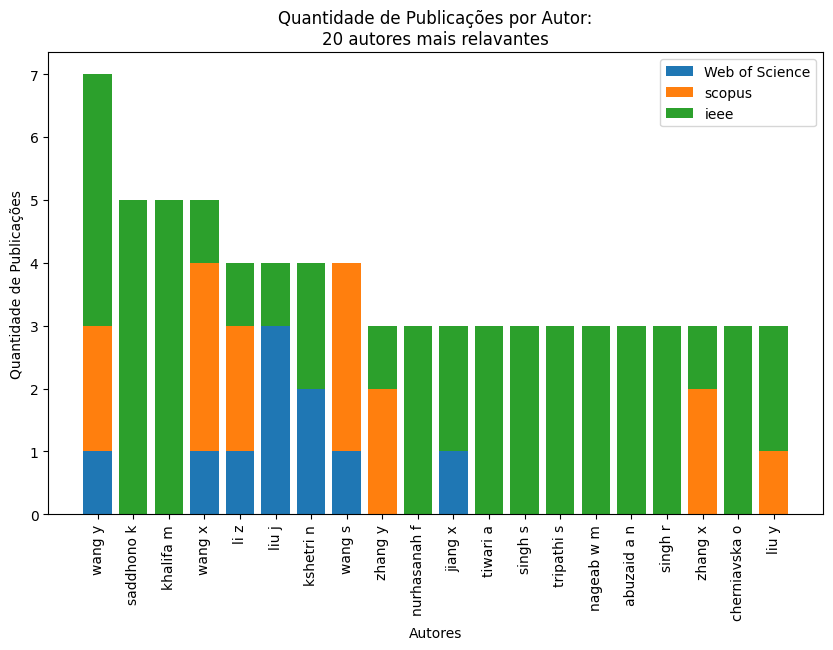
\includegraphics[width=12.5cm]{publicacoes_autores.png}
    \label{fig:4}
    {\\\footnotesize Fonte: Autoria Própria}
\end{figure}

O estudo identificou 2.822 autores distribuídos em 891 artigos\footnote{Alguns registros apresentaram problemas no cadastro dos autores, resultando na redução da base de 907 para 891 publicações}. Conforme explicado por \textcite{melo2017bibliometria}, a produtividade acadêmica frequentemente segue o padrão de Lotka, onde um pequeno número de autores resulta na maior parte das publicações, enquanto a maioria contribui com um ou poucos artigos. Esse padrão é claro na Tabela \ref{tab:2}, que mostra que 2.620 autores publicaram somente um artigo, enquanto um autor singular participou de sete publicações, ressaltando a significativa assimetria na distribuição da produção científica sobre esse tópico.

\begin{table}[H]
    \centering
    %\footnotesize
    \begin{tabular}{cccc}
        \hline
        Qtd. Publicações & Qtd. Autores & Total de Autores & Total de Participações em Publicações \\
        \hline
        \rowcolor{red!30} 7  & 1    & 1    & 7    \\
        \rowcolor{red!30} 5  & 3    & 4    & 22   \\
        \rowcolor{red!30} 4  & 4    & 8    & 38   \\
        \rowcolor{red!30} 3  & 18   & 26   & 92   \\
        \rowcolor{red!30} 2  & 176  & 202  & 444  \\
        1  & 2620 & 2822 & 3064  \\
        \hline
    \end{tabular}
    \caption{Distribuição das publicações por autor.}
    \label{tab:2}
\end{table}

A tabela \ref{tab:2} demonstra que, ao agrupar os autores com base no número total de contribuições em publicações em três categorias de relevância ($3064/3\approx1021.33$), a linha final excedia o critério estabelecido. Esse critério ajudou a minimizar ainda mais a base de dados de publicações, reduzindo o total para 257 artigos considerados relevantes. Assim, também reduziu-se o número total de autores classificados como relevantes de 2822 para 202, estabelecendo que o mínimo de publicações necessário para ser considerado relevante era de duas publicações.

A análise realizada por diversos autores repete a constatação de que o tema em questão continua a apresentar desafios consideráveis, sendo ainda imperativo seu aprofundamento. Ao contrastarmos a curva descendente no número de autores, predita pela equação de Lotka (\ref{eq:lotka}), com o volume de publicações presente na base de dados, nota-se que o número de autores de relevância permanece abaixo do esperado para o tema abordado, conforme ilustrado na Figura \ref{fig:teste_lotka}.

\begin{figure}[H]
    \centering
    \caption{Comparação do volume de publicações por autores da base com a equação de Lotka.}
    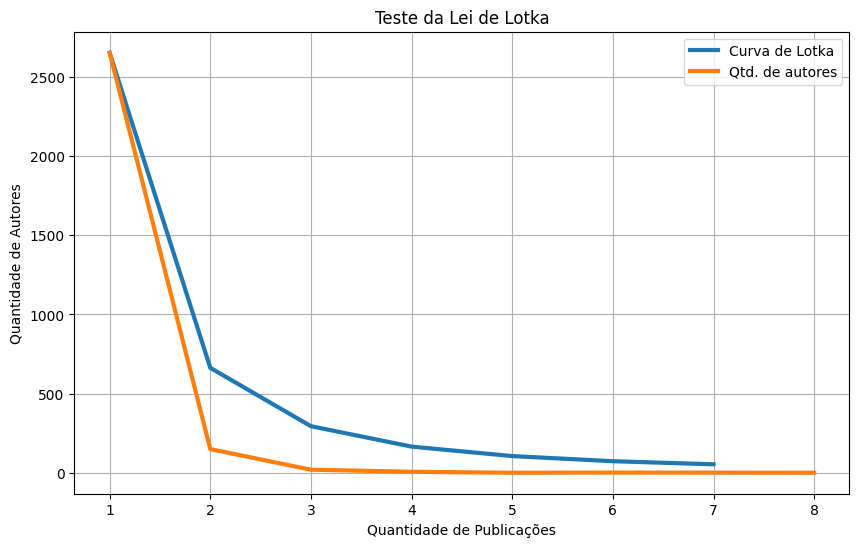
\includegraphics[width=13cm]{teste_lotka.png}
    \label{fig:teste_lotka}
    {\\\footnotesize Fonte: Autoria Própria}
\end{figure}

%***** Análise das palavras utilizadas *****
\subsection{Análise das palavras nos Títulos, Palavras-chaves e Resumos}

Com a redução das bases de dados, visou-se identificar os principais temas discutidos nas publicações escolhidas. Para isso, procedeu-se a uma análise dos títulos, palavras-chave e resumos dos artigos. Em vez de aplicar a Lei de Zipf diretamente, conforme descrito por \textcite{guedes2005bibliometria}, decidiu-se primeiro eliminar elementos estruturais da língua inglesa, tais como conjunções coordenativas e subordinativas, conjunções correlativas, artigos, preposições, pronomes, predeterminadores, verbos auxiliares, pronomes demonstrativos, advérbios e adjetivos possessivos. Essa estratégia assegurou a preservação somente de estruturas linguísticas com maior carga semântica, incluindo substantivos, verbos principais, adjetivos descritivos, numerais e interjeições, o que facilitou a quantificação dos termos mais relevantes. Assim, foi possível deduzir com maior precisão os tópicos predominantes nos artigos analisados.

A Figura \ref{fig:5} exibe a nuvem de palavras criada a partir dos títulos, palavras-chave e resumos dos artigos escolhidos. Nesta representação gráfica, palavras mais recorrentes são destacadas em comparação com outras. Para melhorar a análise, termos intrinsecamente ligados ao escopo da pesquisa, como \textit{artificial, intelligence, AI, generative} e \textit{impact}, foram omitidos, já que são resultado direto da seleção dos artigos. Nota-se, no entanto, a presença de termos associados a diversas áreas do conhecimento, como educação, tecnologia, marketing, mercado e literatura. Além disso, a identificação de substantivos menos comuns, como desafios, ética, avaliação e potencial, destaca aspectos críticos e impactos significativos dessa tecnologia em vários contextos.

\begin{figure}[H]
    \centering
    \caption{Totalização das palavras: Títulos, Palavras-Chave e Resumos}
    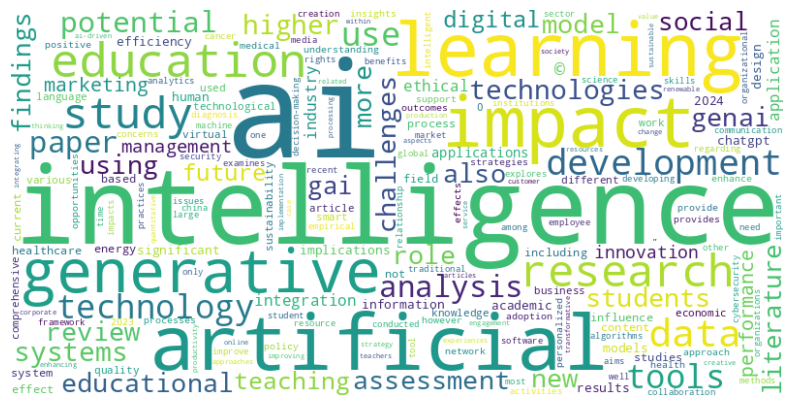
\includegraphics[width=13cm]{nuvem_palavras.png}
    \label{fig:5}
    {\\\footnotesize Fonte: Autoria Própria}
\end{figure}

Ao analisarmos a Figura \ref{fig:5}, observamos que o tema relacionado à educação se destaca nos artigos selecionados. Portanto, foi realizada uma filtragem mais específica, incluindo essa palavra nos títulos, resumos e palavras-chave. O resultado dessa filtragem totalizou 19 artigos, como apresentado na Tabela \ref{tab:3}\footnote{Ao examinar os títulos e autores, observa-se a utilização somente de letras minúsculas. Esta técnica é empregada para classificar as publicações ao longo da aplicação da metodologia.}

\begin{longtable}{|p{10cm}|p{6cm}|}
    \hline
    \textbf{Título} & \textbf{Autores} \\ 
    \hline
    artificial intelligence in education: a promise, a threat or a hype? & humble n, mozelius p \\
    \hline
    artificial intelligence in education: implications for academic integrity and the shift toward holistic assessment & atieeq a, zoraki m, milhem m, atieeq ra \\
    \hline
    exploring the impact of artificial intelligence generative tools on research in higher education institutions: a perspective from portugal & sobral s r, ferreira m j, pereira c s, durão n, moreira f \\
    \hline
    the role of generative artificial intelligence (gai) in education: a detailed review for enhanced learning experiences & kumar t, ankita, malik s \\
    \hline
    enhancing higher education in portugal: leveraging generative artificial intelligence for improved learning-teaching process & pereira c s, ferreira m j, sobral s r, durão n, moreira f \\
    \hline
    exploring the potential of chatgpt to improve experiential learning in education & rawat s, mittal s, nehra d, sharma c, kamboj d \\
    \hline
    exploring students foundational skills in integrating generative ai in ghanaian higher education: a constructive learning perspective & adam i o, alhassan m d, diack a \\
    \hline
    a scoping review on how generative artificial intelligence transforms higher education & xia q, ouyang f, lin t j, chiu t k f \\
    \hline
    generative ai in higher education: seeing chatgpt through universities' policies, resources, and guidelines & wang h, wu z, mac s \\
    \hline
    demystification of generative artificial intelligence (ai) literacy, algorithmic divide, pedagogical knowledge: a comprehensive model & dadhich m, haumik a \\
    \hline
    empowering academic success: integrating ai tools in university teaching for enhanced assignment and thesis guidance & atieeq a, alzoraiki m, milhem m, b a hasan beshr \\
    \hline
    enhancing educational outcomes through exploring the optimized options artificial intelligence and deep learning & legowo b, nurhasanah f, saddhono k, budiastuti v i, sutomo a d, murwaningsih t \\
    \hline
    an evaluation of ai-enhanced collaborative learning platforms & islam a, ali j \\
    \hline
    enhancing predictive analytics in education through collaborative filtering algorithms in knowledge management & tastanova m, jilkibaeyva z, arkhabayeva z, tripathi s \\
    \hline
    harnessing potential: meta-analysis of ai integration in higher education & a m a samman \\
    \hline
    an integration of ai and traditional methodology in the education field in order to: transform the trends & marmoah s, murwaningsih t, nurhasanah f, saddhono k, sutomo a d, legowo b \\
    \hline
    the use of artificial intelligence techniques in smart classrooms is in its infancy & figueroa e, batista e, palau r, unciti o, ferre m, martinez-ballesté a \\
    \hline
    the best of way of using ai technology in designing technical education curriculum in meeting future industry demands: smart way & s h m issa, saddhono k, sarwanto, a s c nugraheni, nurhasanah f \\
    \hline
    smart system with leveraging ai integrating system for well designed learning system & rahardjo s, marmoah s \\
    \hline
    \caption{Relação de Artigos selecionados com o tema de \textit{Education}.}
    \label{tab:3}
\end{longtable}

%************************
% Considerações Finais **
%************************
\section{Considerações Finais}
%\onehalfspacing
 Este estudo realizou uma análise bibliométrica abrangente das Inteligências Artificiais Generativas (IAGs), destacando avanços científicos e desafios enfrentados pela comunidade acadêmica. Utilizando metodologias quantitativas, como as leis de Bradford, Lotka e Zipf, foi possível identificar padrões de disseminação do conhecimento, principais periódicos e autores mais produtivos, além das áreas de conhecimento impactadas por essas tecnologias \cite{guedes2005bibliometria}. 
 
 A pesquisa revelou um aumento expressivo no volume de publicações sobre IAGs nos anos recentes, evidenciando o crescente interesse nesse campo e a necessidade de uma organização cuidadosa da produção científica. Os resultados mostram que, embora a distribuição da pesquisa sobre IAGs siga padrões compatíveis com as Leis de Bradford e Lotka, a concentração das publicações nos principais periódicos e entre os autores mais produtivos ainda é relativamente baixa. A maior parte dos artigos está dispersa entre um grande número de periódicos e autores que publicaram apenas uma única vez sobre o tema, sugerindo que núcleos difusores e pesquisadores influentes ainda estão se formando. 
 
 Essa situação pode ser atribuída à recente ascensão das IAGs, resultando em um cenário acadêmico ainda fragmentado. Contudo, a análise dos dados indica que estas concentrações estão começando a se consolidar, sugerindo uma potencial estruturação futura da produção científica sobre o tema. A análise dos títulos, palavras-chave e resumos permitiu identificar principais temas abordados nas publicações. Identificaram-se fortes correlações entre IAGs e áreas como educação, tecnologia, marketing e mercado, além da recorrência de termos relacionados a desafios éticos e metodológicos, como avaliação, potencial e impacto. Essa análise semântica auxilia na identificação de tendências emergentes e lacunas na literatura, fornecendo direção para futuras pesquisas.
 
\printbibliography

\end{document}
